\chapter{Development}

Below is the process of developing a glucose monitoring app using the FreeStyle Libre FGM sensor, which involved reverse engineering the protocol of the Libre, and developing a system for calibration and conversion of raw sensor and temperature values into readings. The application also features speed improvements over current state of the art, and is designed to be open source to function as a platform for building predictive and analytics tools based on such data, in addition to data aggregation.

\section{Architecture}

\begin{figure}[ht]
\centering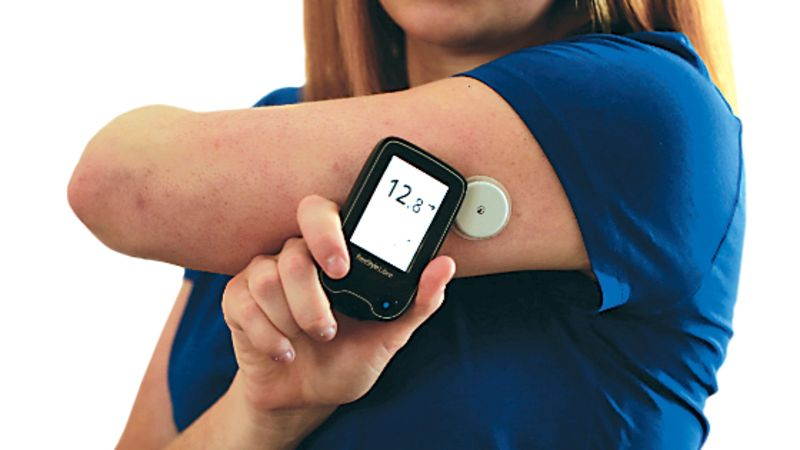
\includegraphics[width=0.4\linewidth]{images/libre1}
\caption{Freestyle Libre sensor and reader in use\cite{noauthor_how_2017}.}
\label{fig:libre1}
\end{figure}

The sensor used in the Freestyle Libre (hereafter referred to as \textit{the sensor} for brevity) is described in multiple patents\cite{noauthor_patents_nodate}, which outline the design and electrochemical composition of the system. Figure~\ref{fig:libre1} shows the scale of the sensor and the reader. Most relevant here are the ones that describe the sensor chemistry as well as notes on the encoding patterns. The chemical method being used\cite{say_electrochemical_2000} is described to vary linearly with temperature as well as the concentration of interstitial fluid glucose. The raw values thus extracted from the electrode on the sensor are then stored in a processing unit on the sensor, as underlined by the patent. 

\begin{figure}[ht]
\centering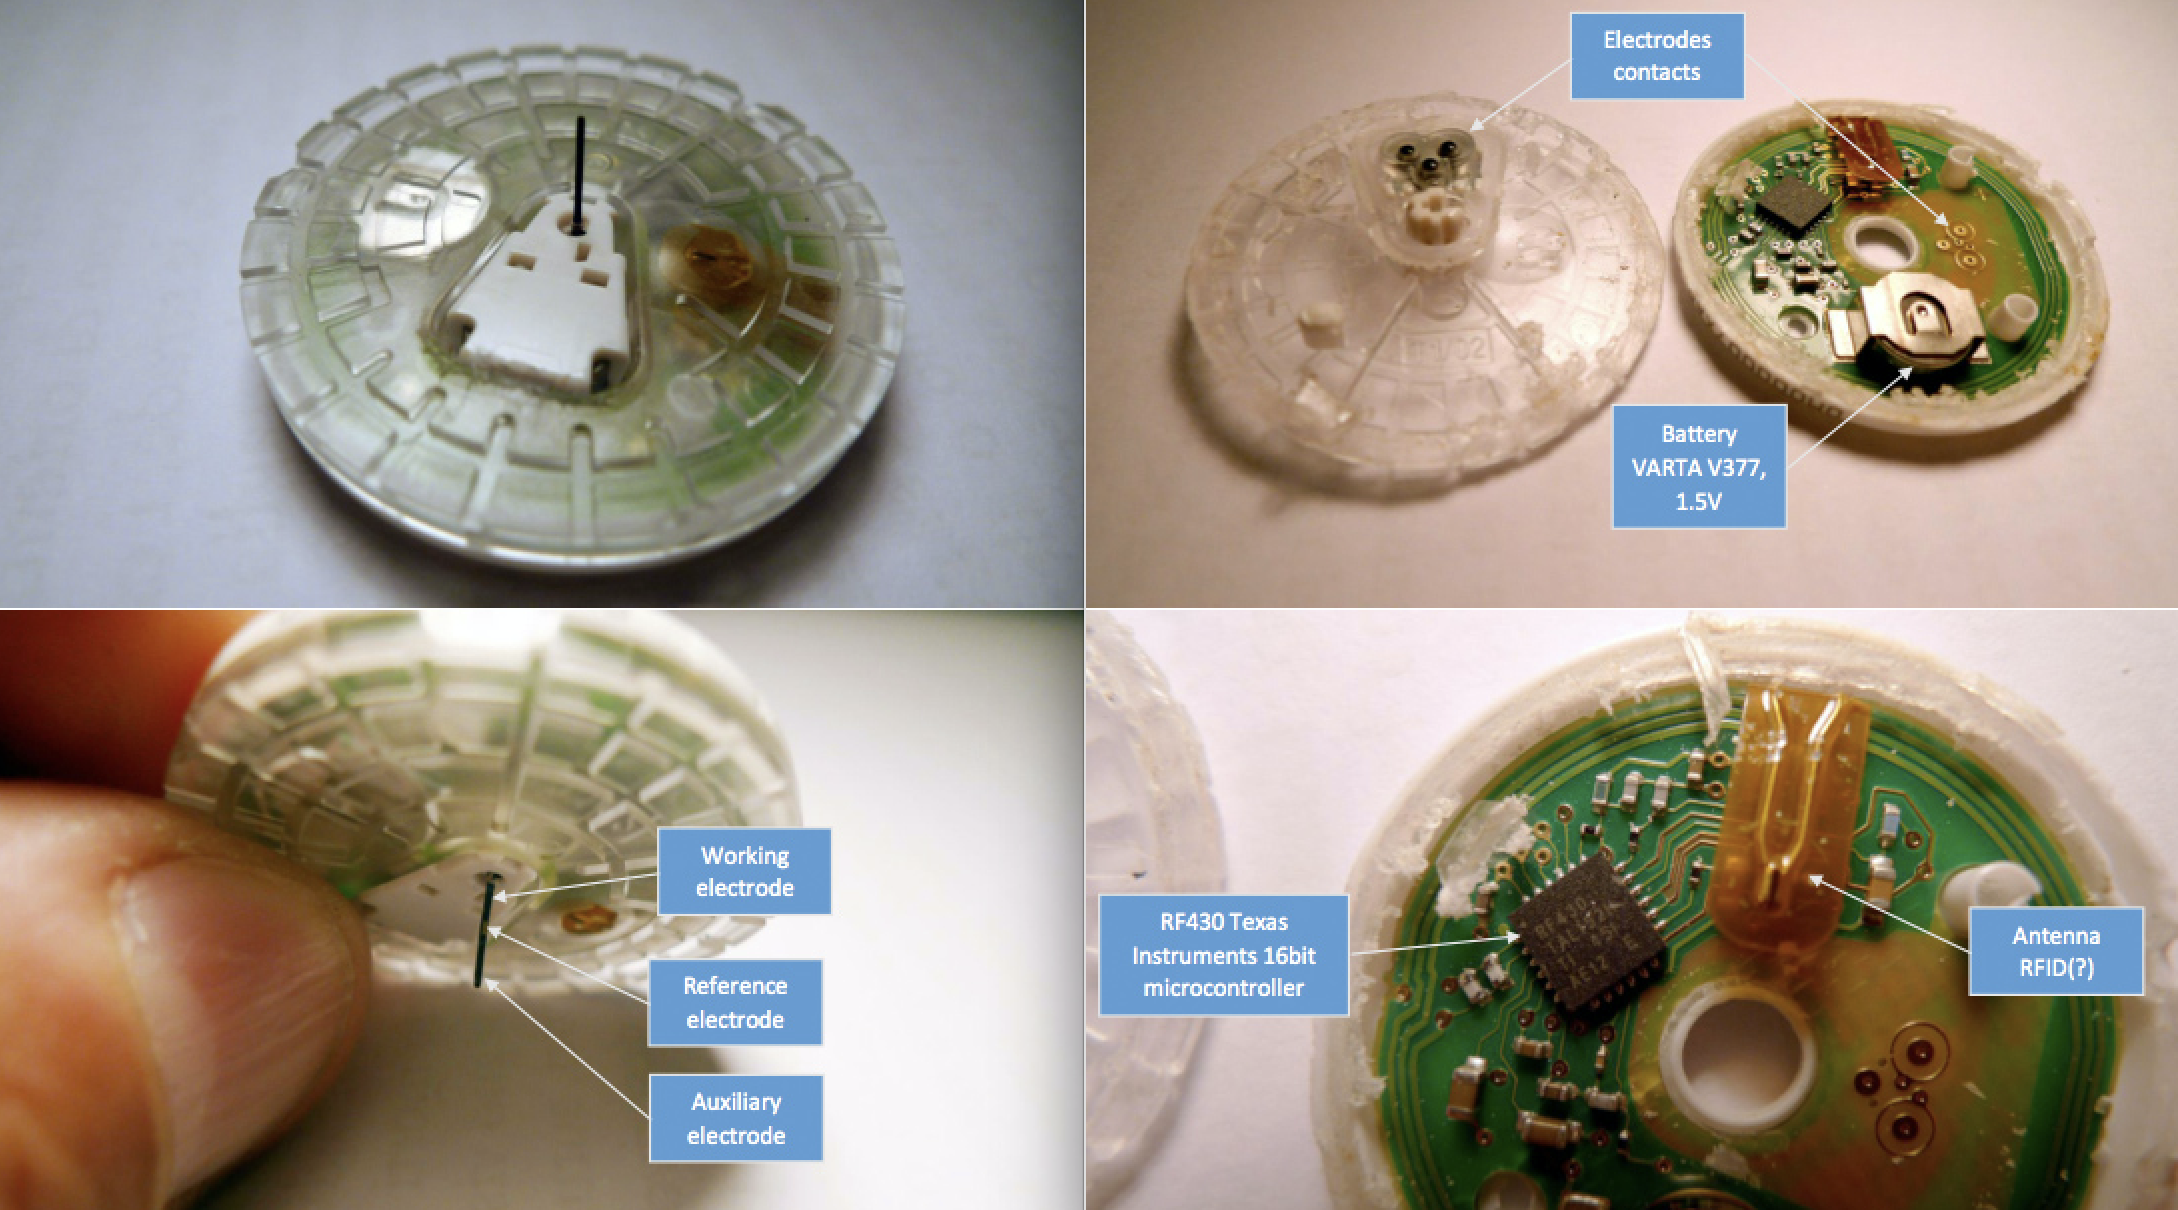
\includegraphics[width=1.0\linewidth]{images/libre4}
\caption{External and internal components of the sensor\cite{ilka_freestyle_2014}.}
\label{fig:libre2}
\end{figure}

A teardown view of the sensor is presented in Figure~\ref{fig:libre2}, where the processor being used as well as the internal components can be identified. The sensor apparatus uses a thermocouple tape\cite{noauthor_thermocouple_1971} which reacts linearly(within thresholds underlined in the patent) to temperature. Single-point and dual-point calibration systems are mentioned, by the use of which the raw sensor glucose information can be calibrated to the internal temperature of the sensor. The only visible temperature sensor\footnote{It must be noted that the processor carried an on-board temperature sensor. However, it is unknown how this is used.} is on-board the sensor body, taped to the plastic housing on the side of the user's skin. This leads us to believe that a single-point calibration is being used, which will be confirmed later.

The processor (from the product number) is an  RF430FRL152H\cite{noauthor_rf430frl152h_nodate}
\footnote{a member of the MSP430\cite{noauthor_16-bit_nodate} family of low-power microcontrollers by Texas Instruments}, which is used to read and store raw values from the sensor, and communicate them over a Near-Field Communication(NFC)\cite{noauthor_near-field_2017} protocol to the reader apparatus. Unfortunately there are no accessible debugging points on the circuit board, so most of the work will need to be done through the wireless protocol on board.

An on-board battery powers the sensor during operation, however, the patent does not describe any mechanisms for calibrating the voltage drift from the battery provided DC voltage. This was surprising, and leaves potential room for additional work on whether this is a factor.

\begin{figure}[ht]
\centering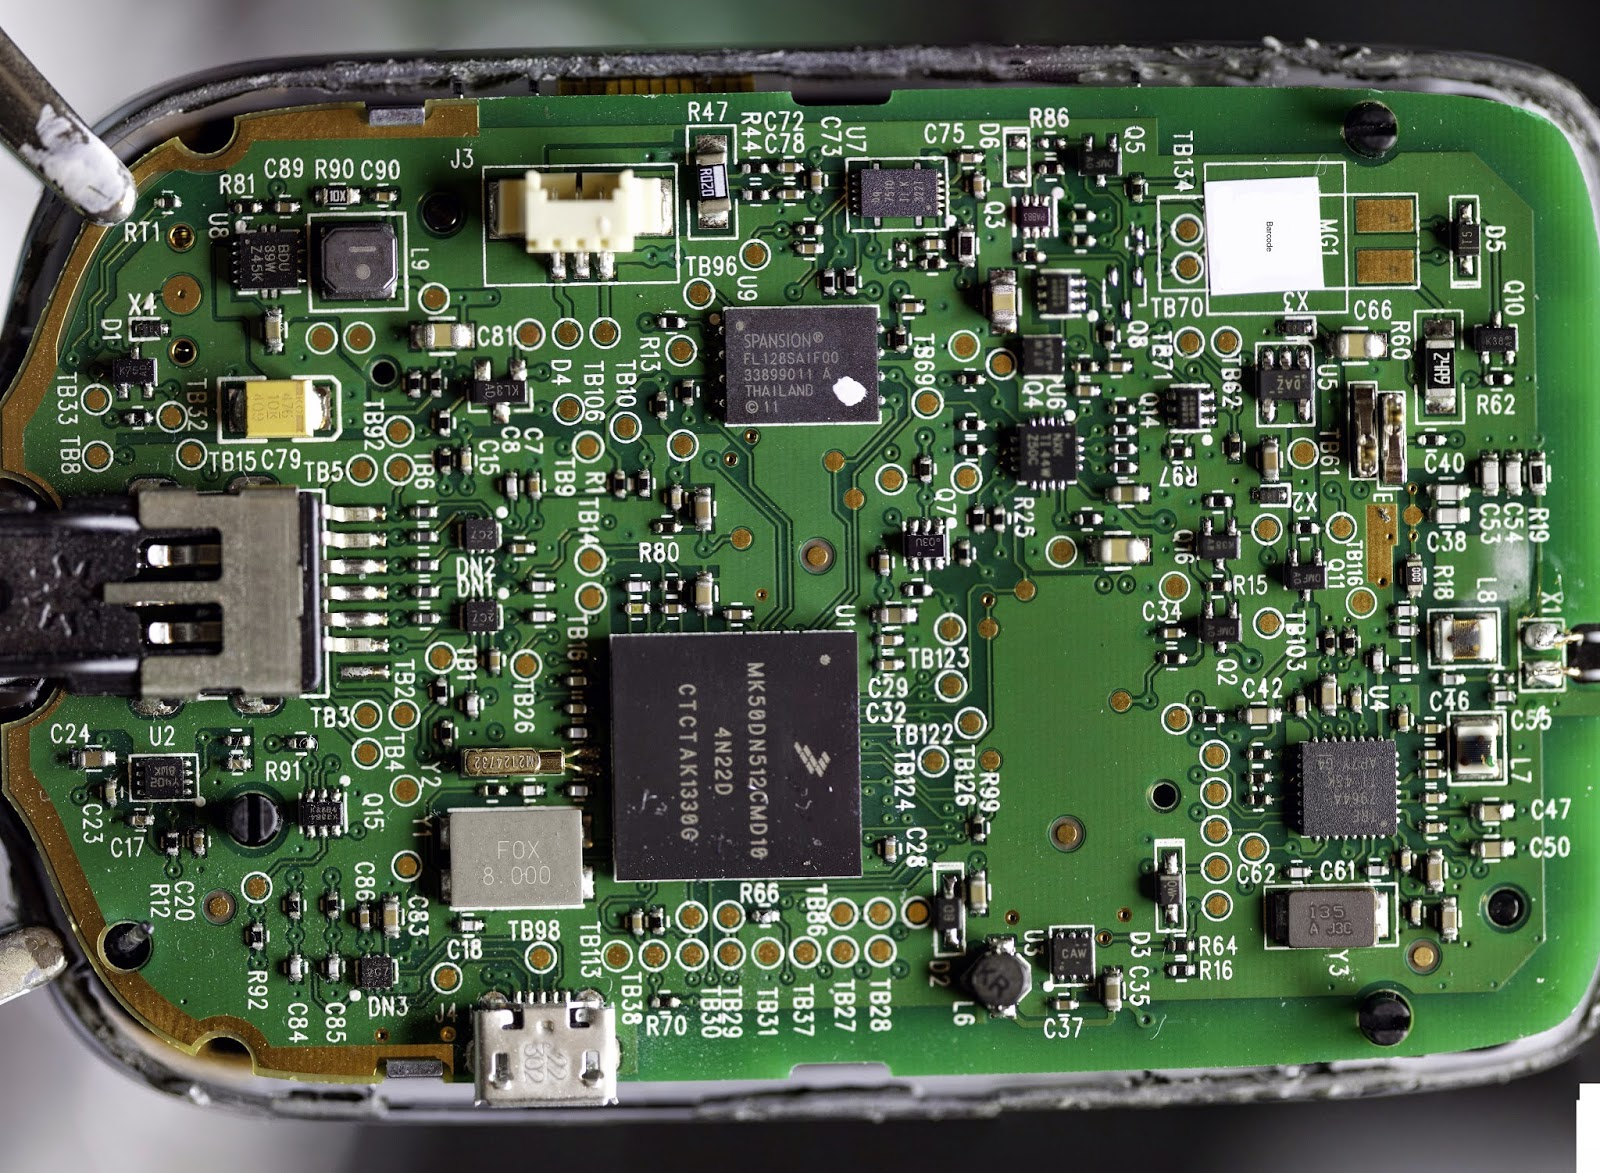
\includegraphics[width=1.0\linewidth]{images/libre5}
\caption{Internal PCB of the reader\cite{noauthor_type_nodate}.}
\label{fig:libre3}
\end{figure}

The reader apparatus (Figure~\ref{fig:libre3}) unsurprisingly complex, as it incorporates the mechanism for reading and processing sensor data, USB interfacing components as well as a blood-glucose test strip reader. The internals are protected weatherproofed, and the construction is remarkably robust. The existence of a number of test pads (possibly for in-factory calibration and quality control as well as an unexposed connector leave future avenues for extraction information from the reader).

\section{Communication Protocol Analysis}

The datasheet\cite{noauthor_rf430frl152h_nodate} for the on-board processor of the sensor describes use of the ISO 15692\cite{noauthor_iso/iec_2017} protocol, and reading the information using an NFC reader application on an Android phone confirms that it conforms to the Nfc-V\cite{noauthor_nfcv_nodate} standard, which is a distance-limiting version of the ISO protocol. This limits the effective use of a reader apparatus to a few centimeters\cite{noauthor_nfc_nodate}, but also requires that all new Android smartphones with Nfc technology be able to read them. The manufacturer is listed as Texas Instruments, with 1952 bytes of memory being transmitted on a full read. Armed with this information, we can proceed.

\subsection{Related Work}

A number of projects have attempted to use the Freestyle Libre as a Continuous Glucose Monitor. There have also been a number of attempts to reverse engineer the protocol being used and to extract the values therein. The most popular (with about 50,000 downloads) of which is the Android application Glimp\cite{software_glimp_2017}, which reads the FreeStyle Libre sensor and claims to "calibrate" the sensor using Blood Glucose readings independently provided by the user. Unfortunately, this project is not open source, and the available open source offerings do not go further than reading raw glucose values without calibration or temperature data, and suffer from long read-times(exceeding 2 seconds) for the sensor. Users have also reported that the measurements thus provided are often wrong, and often dangerous - in fact, as one particular analysis shows, the calibration methods used lead to often fatal predictions for users\cite{v_libre_nodate}. The closest project that could be found was the FreeStyleLibre-NFC-Reader\cite{bautista_freestylelibre-nfc-reader:_2017} project, which displayed the most recently recorded sensor value\footnote{Small caveat being that the code was largely uncommented and labeled in Spanish.}. Looking at available solutions for working with the FreeStyle Libre system indicated the dire need for open source projects that aim to improve on intelligent reporting as well as detailed documentation on internal working.

The accompanying Wiki article was useful in providing the following information:

\begin{enumerate}
\item The glucose data being recorded on the sensor is split into 16 measurements spaced one minute apart and 32 measurements spaced 15 minutes apart.
\item A circular array is used for writing the data (presumably to minimize rewrites to memory), and the next write position is recorded in the hex before the two arrays.
\item The numbers are encoded in Little Endian Binary\cite{noauthor_endianness_2017}.
\end{enumerate}

However, the author states that his analysis is purely experimental, and that it fails on a sensor that is in use for more than 10 days (the labeled use period of the sensor is 14 days). However, this provides a suitable starting point if we proceed with caution.

\section{HEX Analysis}

\begin{figure}[ht]
\centering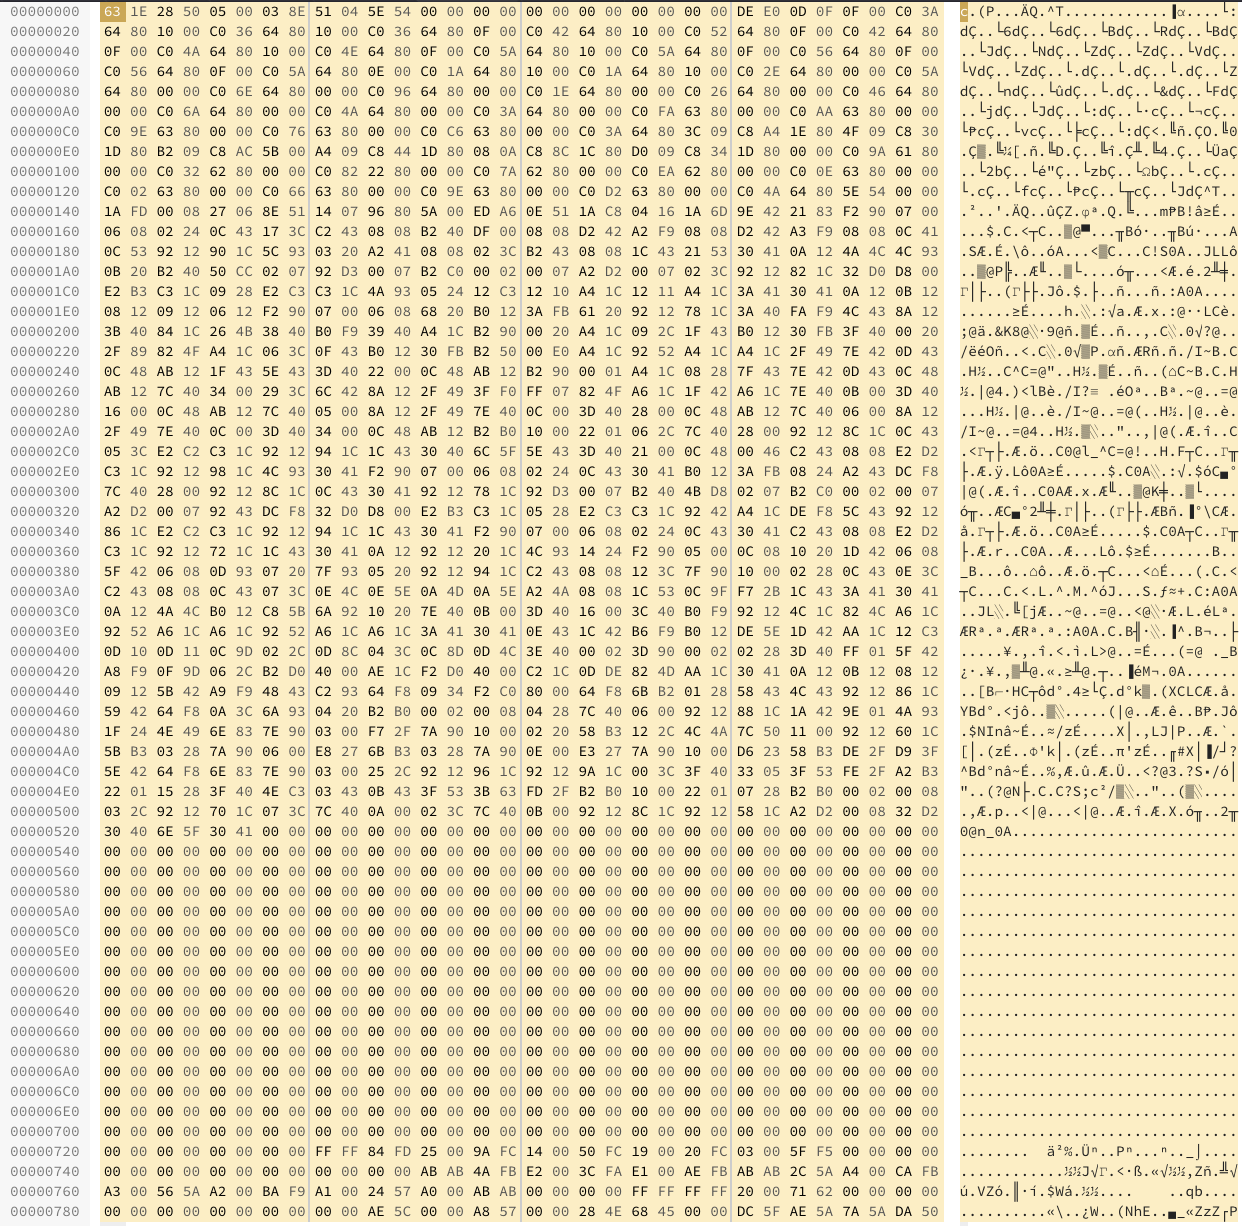
\includegraphics[width=0.5\linewidth]{images/hexdump.png}
\caption{Full hexadecimal and ASCII character dump of sensor tag memory.}
\label{fig:hexdump}
\end{figure}

Visual analysis of the tag memory indicates that a large amount of whitespace remains (Figure~\ref{fig:hexdump}), and comparing to sensor read times for the full tag as opposed to existing solutions (Glimp, Liapp, etc), we can predict that reading only the required bits of the sensor will let us speed up this process considerably.

A python program\footnote{processrawNFC.py in source code} to process the resulting XML and convert it to an addressable array of hex values enables analysis. Considering a differential of consecutive sensor data dumps, we can see the bytes that differ. 

\begin{figure}[ht]
\centering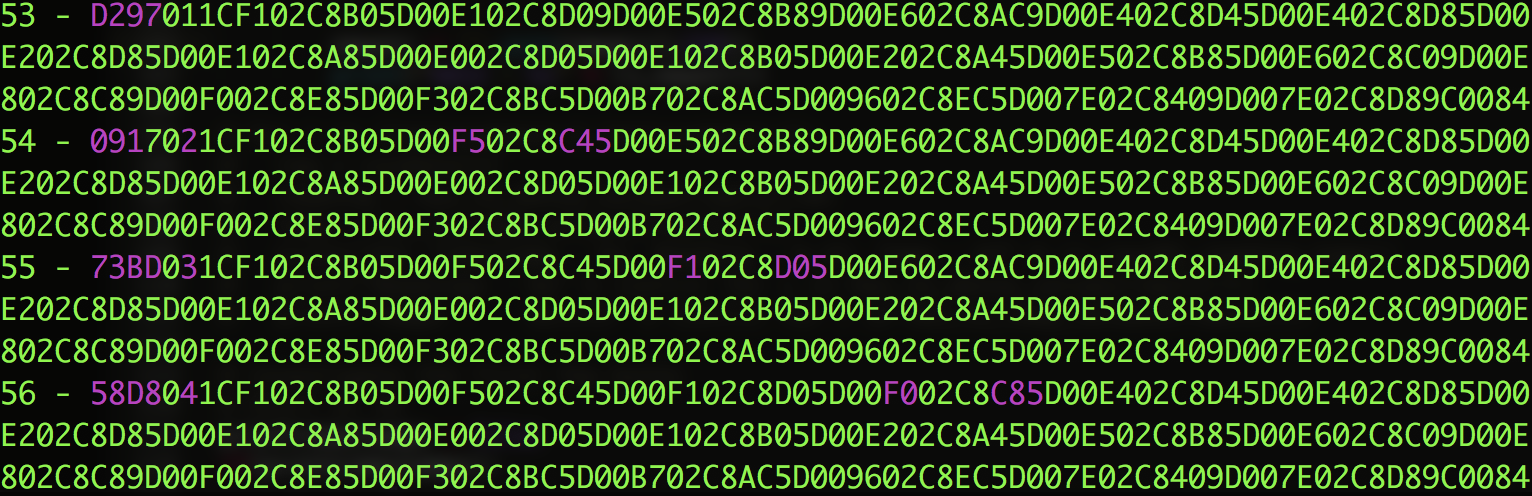
\includegraphics[width=1.0\linewidth]{images/diff.png}
\caption{Differential of sensor hex dumps, with differing bits highlighted in pink.}
\label{fig:diff}
\end{figure}

Figure~\ref{fig:diff} shows hex dumps collected approximately spaces 1 minute apart, which confirm and locate the spots where readings are written. From here, we can take consecutive readings to determine the location of each individual reading, until the write array returns to the same location.

Once this was completed, research suggested that the written values were a combination of flags, raw glucose data and temperature data. What remained was to separate them. This proved simple - removing the sensor from it's position in the body (after insertion and calibration by the reader) provided consistent glucose readings of -21. Given that this was a constant factor, binary analysis revealed that the glucose values were encoded in the lower 3 bytes of the reading, and could be deciphered using Equation \ref{eq:glucoseeq}.

\begin{equation} \label{eq:glucoseeq}
V_{glucose} = \frac{V_{raw}\;\mathrm{\&\; 0x000FFF}}{6}-37 
\end{equation}

Next, the glucose information was calibrated using previously collected raw glucose data from Glimp\cite{software_glimp_2017} which could be matched with processed data extracted from the reader using protocols defined in the open source project Glucometer-protocols\cite{petteno_glucometer-protocols:_2017}. The raw and calibrated data seemed to possess mostly a first order aka linear correlation across sensors (Figure~\ref{fig:corr}, and the value of intercept and slope were used to further adjust raw data collected.

\begin{figure}[ht]
\centering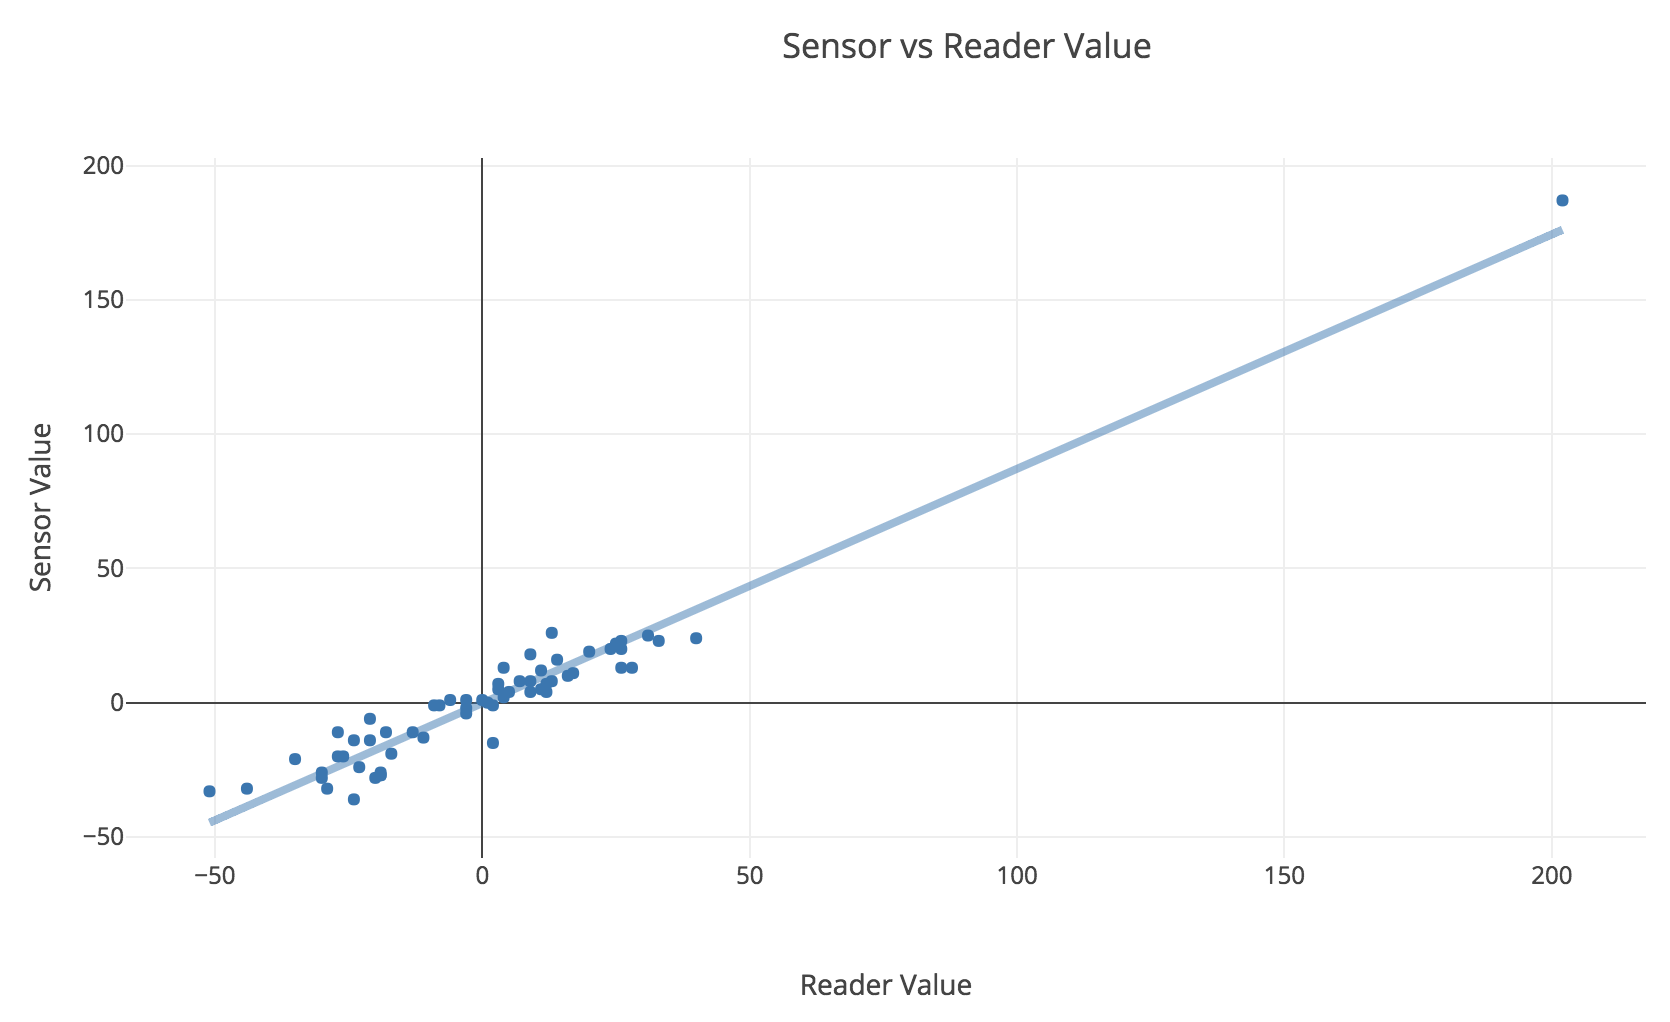
\includegraphics[width=1.0\linewidth]{images/sensorvsreader.png}
\caption{Graph of raw sensor vs processed reader glucose values.}
\label{fig:corr}
\end{figure}

Next was the process of extracting and calibration temperature sensor information. A simple experimental setup of using a multimeter thermocouple taped to the sensor (which was placed closest to the external thermocouple in Figure~\ref{fig:libre2}), following which the apparatus was placed in multiple temperature systems, the average of which was calculated. Once again, the datasheet~\cite{noauthor_rf430frl152h_nodate} was helpful in expecting a linear correlation between temperature and raw values, so a slope, intercept, and a bitmask for the flags was all that was required.

Graphing the resulting data revealed certain flags being turned on and off, which combined with the knowledge that a flag change could be removed with a power of 2, resulted in the bitmask being set at \textbf{0x2FFF}, applied to the upper three bytes of the six-byte reading extracted (the same value can be applied to the entire reading, left shifted). The experimental setup and bitmask evaluation can be found in Figure~\ref{fig:tempcalsetup}.

\begin{figure}[ht]
\centering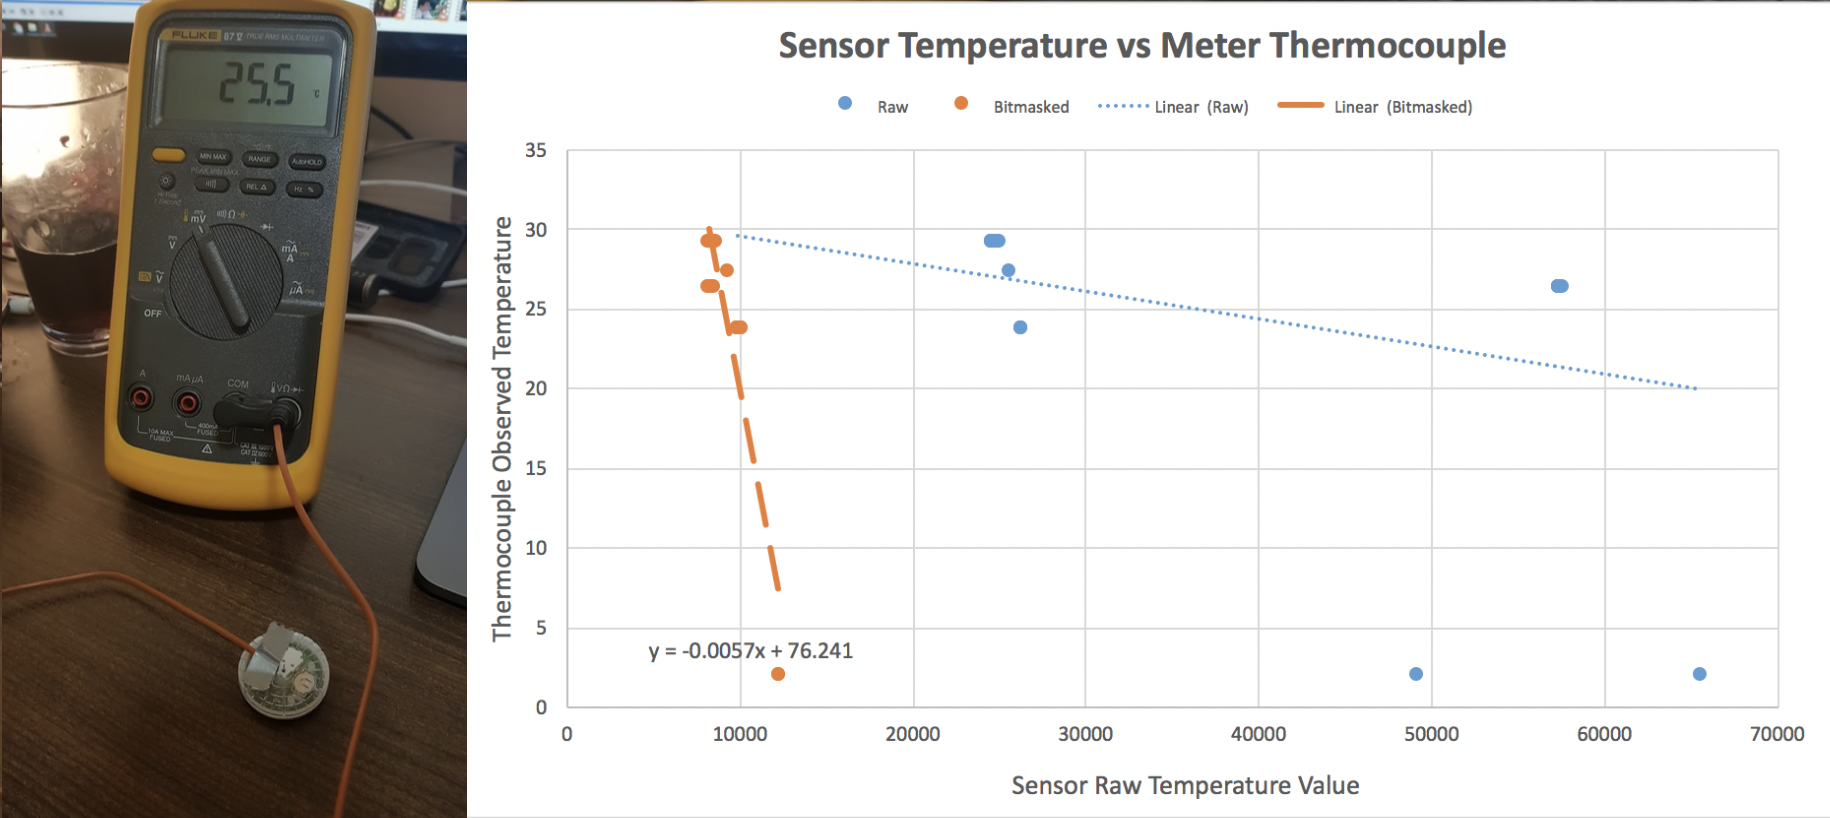
\includegraphics[width=1.0\linewidth]{images/tempcalsetup.png}
\caption{Experimental Setup and bitmasking results of Temperature Calibration.}
\label{fig:tempcalsetup}
\end{figure}

Next, the setup was placed in more accurate ovens that provided better temperature references. In each case, the entire apparatus was placed for a period of 16 minutes. This was due to the uncertainty of the sensor's reading within a minute. Once all previous short term memory had been overwritten, the average of these results along with the average of the meter reading was used to create a calibration line to find the slope and intercept\footnote{The meaning of flags were not ascertained due to time constraints and limited testing conditions, and was left for future work.}. 

\begin{figure}[ht]
\centering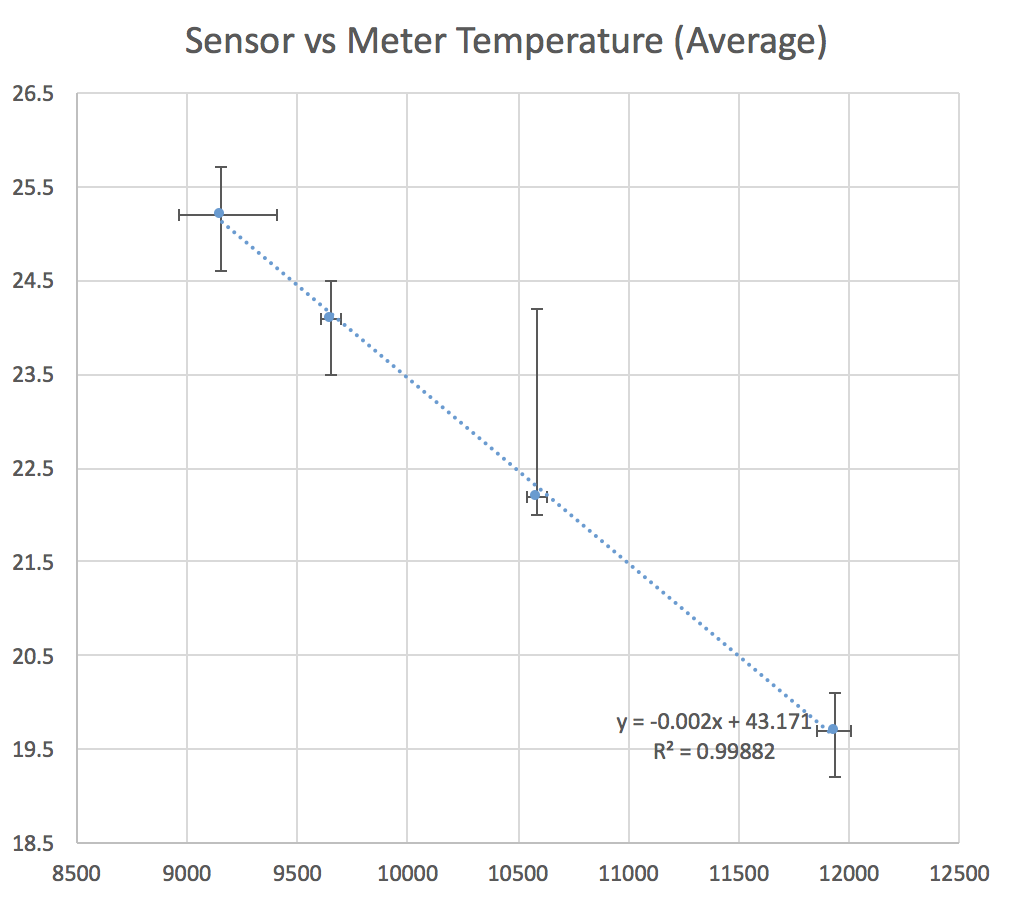
\includegraphics[width=0.75\linewidth]{images/tempcal2.png}
\caption{Detailed calibration of temperature values.}
\label{fig:tempcal2}
\end{figure}

Figure~\ref{fig:tempcal2} shows how the raw sensor values were related to measured temperature values from the meter. Once the bitmask was applied, the linear relationship was evident.

\section{Application Development}

The next step involved developing an Android application using the information found through reverse-engineering the NfcV protocol. The standard Java stack for Android was used, and the resulting application can be seen in Figure

Some optimizations were made to increase read times beyond state-of-the-art. From a preliminary study, current solutions were unable to get sensor scan times less than 1.5 seconds. This was found to be due to the large memory of the NfC chip in the sensor, and the slow read times of the protocol. Information could only be read in packets of eight bytes - scanning the entire chip took over five seconds, and reading valid program memory took over a second.

Reverse engineering the Glimp app (which provided no source code) allowed for decrypting the sensor tag label from the metadata provided by the sensor. The full algorithm is shown in Figure~\ref{fig:sensortagalgo}. The Libre sensor uses a reduced set of alphanumeric characters and some form of compression to encode the sensor label that is printed on the side of each device.

\begin{figure}[ht]
\centering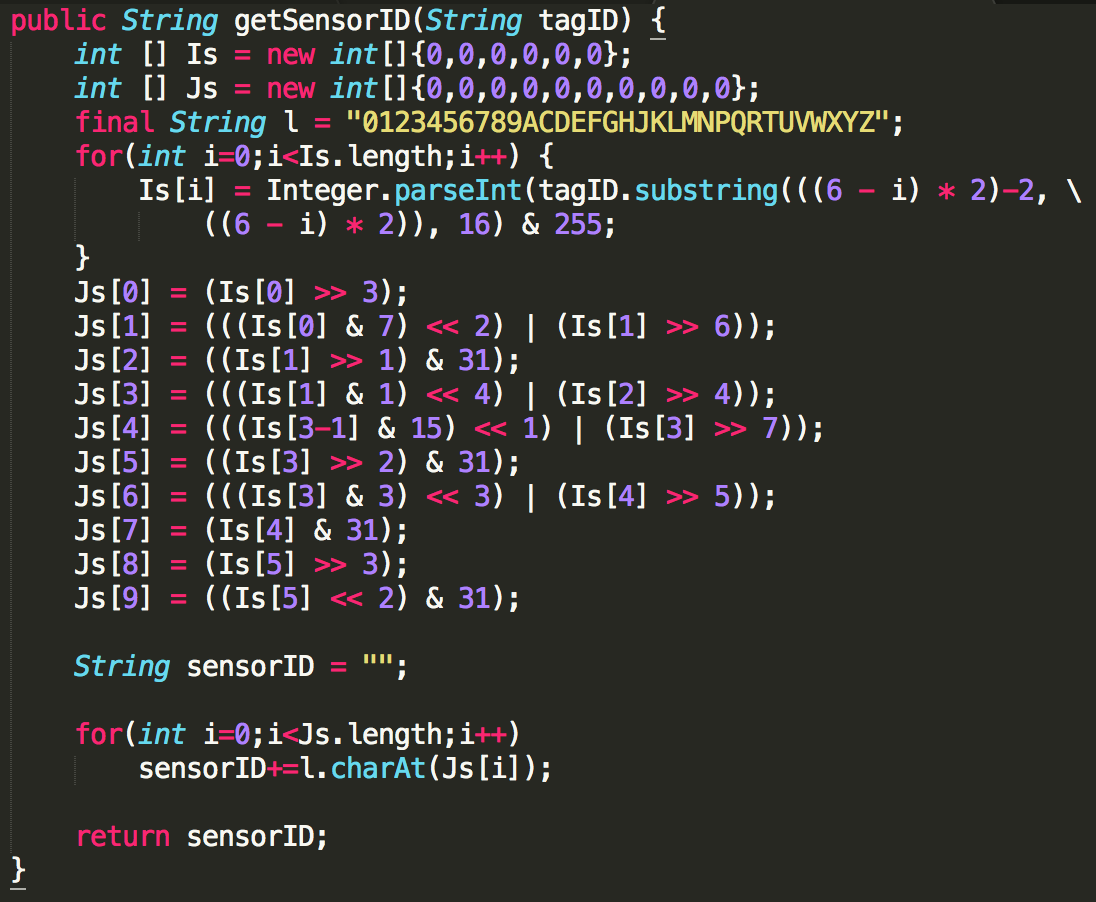
\includegraphics[width=0.75\linewidth]{images/sensortagalgo.png}
\caption{Algorithm used to decrypt sensor tag information.}
\label{fig:sensortagalgo}
\end{figure}

Using this data, it was possible to match previously read values to the values being presently read, and to stop when a previously known value was encountered. This greatly reduced read times by removing the need to read the entire memory, or even the entire array of values. For a subsequent read of the same sensor within 60 seconds, the total read time was less than 50 ms, which only included the time it took to read one short term value and one long term to confirm. On average, read times were decreased to less than 500 ms, which provided a significant advantage over existing apps and systems. The only known faster scanning system is the physical reader provided by Abbott, making this a competitive option due to low cost and greater accessibility.